\documentclass[border=6pt]{standalone}
\usepackage{tikz}
\usetikzlibrary{arrows.meta,positioning,fit,calc}
\definecolor{fg}{HTML}{DBC9A8}
\definecolor{fgbody}{HTML}{C4A882}
\definecolor{stroke}{HTML}{C4963C}
\definecolor{surf}{HTML}{22222B}
\definecolor{surfemph}{HTML}{2A2820}
\definecolor{surfact}{HTML}{2E2020}
\definecolor{bdim}{HTML}{9A7F62}
\definecolor{bemph}{HTML}{D4A849}
\definecolor{bact}{HTML}{FF5C5C}
\begin{document}
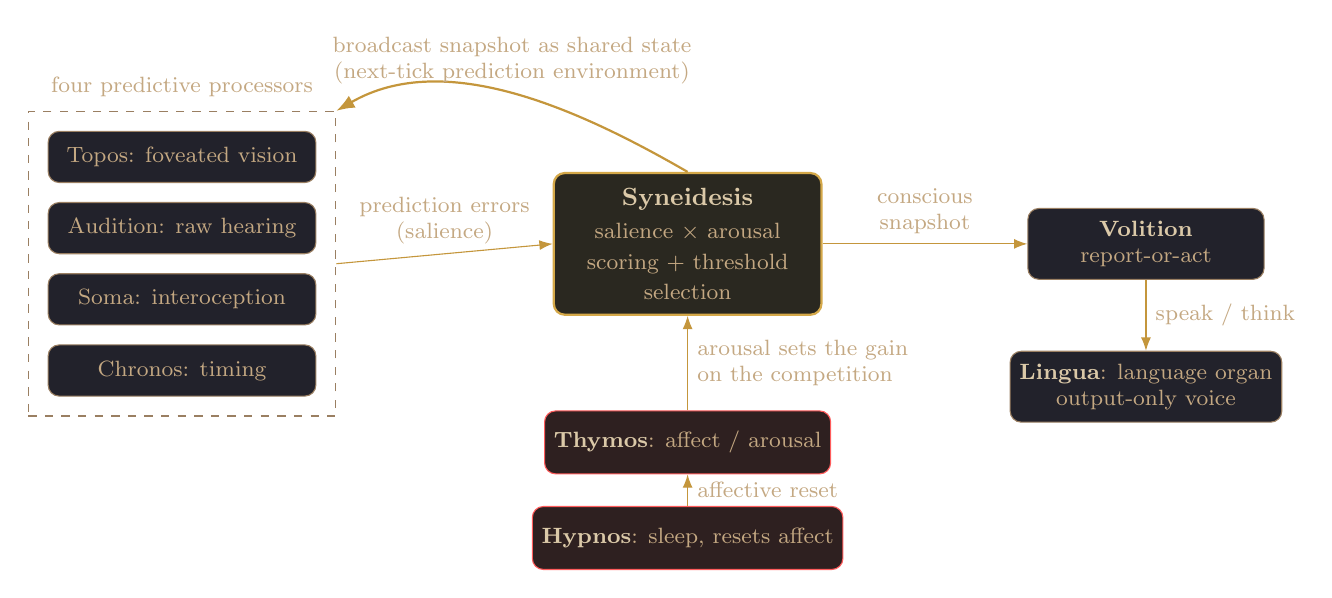
\begin{tikzpicture}[
  font=\small,>=Latex,
  mod/.style={draw=bdim, rounded corners, fill=surf, text=fgbody, align=center, minimum width=34mm, minimum height=6.5mm, font=\footnotesize},
  aff/.style={draw=bact, rounded corners, fill=surfact, text=fgbody, align=center, minimum width=34mm, minimum height=8mm, font=\footnotesize},
  work/.style={draw=bemph, thick, rounded corners, fill=surfemph, text=fgbody, align=center, minimum width=34mm, minimum height=18mm},
  act/.style={draw=bdim, rounded corners, fill=surf, text=fgbody, align=center, minimum width=30mm, minimum height=9mm, font=\footnotesize},
]
% four predictive processors on the left
\node[mod] (m1) {Topos: foveated vision};
\node[mod, below=2.4mm of m1] (m2) {Audition: raw hearing};
\node[mod, below=2.4mm of m2] (m3) {Soma: interoception};
\node[mod, below=2.4mm of m3] (m4) {Chronos: timing};
\node[draw=bdim, dashed, fit=(m1)(m2)(m3)(m4), inner sep=7pt] (mods) {};
\node[font=\footnotesize, text=fgbody, above=0.5mm of mods] {four predictive processors};
% workspace centre
\node[work, right=30mm of m2, yshift=-2mm] (syn) {\textcolor{fg}{\textbf{Syneidesis}}\\[1pt]\footnotesize salience $\times$ arousal\\\footnotesize scoring $+$ threshold\\\footnotesize selection};
% affect below the workspace
\node[aff, below=12mm of syn] (aff) {\textcolor{fg}{\textbf{Thymos}}: affect / arousal};
\node[aff, below=4mm of aff] (hyp) {\textcolor{fg}{\textbf{Hypnos}}: sleep, resets affect};
% report-or-act and the language organ on the right
\node[act, right=26mm of syn] (vol) {\textcolor{fg}{\textbf{Volition}}\\report-or-act};
\node[act, below=9mm of vol] (lin) {\textcolor{fg}{\textbf{Lingua}}: language organ\\output-only voice};
% modules -> workspace (errors)
\draw[->, draw=stroke] (mods.east) -- node[above, font=\footnotesize, align=center, text=fgbody]{prediction errors\\(salience)} (syn.west);
% affect -> workspace (precision)
\draw[->, draw=stroke] (aff) -- node[right, font=\footnotesize, align=left, text=fgbody]{arousal sets the gain\\on the competition} (syn);
% hypnos -> thymos
\draw[->, draw=stroke] (hyp) -- node[right, font=\footnotesize, text=fgbody]{affective reset} (aff);
% broadcast loop back over the top
\draw[->, thick, draw=stroke] (syn.north) to[out=150,in=30,looseness=0.9] node[above, font=\footnotesize, align=center, text=fgbody]{broadcast snapshot as shared state\\(next-tick prediction environment)} (mods.north east);
% workspace -> volition
\draw[->, draw=stroke] (syn) -- node[above, font=\footnotesize, align=center, text=fgbody]{conscious\\snapshot} (vol);
% volition -> lingua
\draw[->, draw=stroke] (vol) -- node[right, font=\footnotesize, text=fgbody]{speak / think} (lin);
\end{tikzpicture}
\end{document}
